\subsection{Our Parallel Louvain implementation}
\label{sec:louvain}

\begin{figure}[hbtp]
  \centering
  \subfigure{
    \label{fig:louvainrak-pruning--all}
    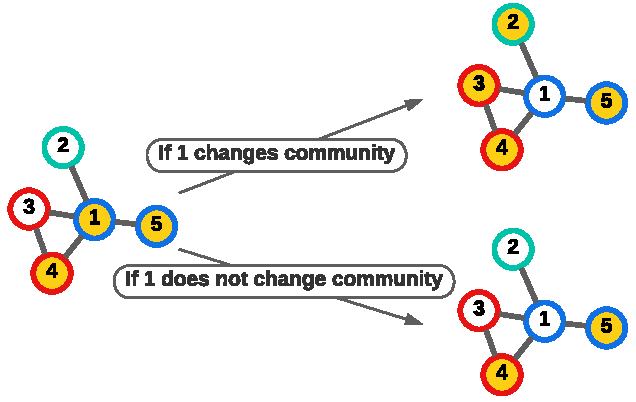
\includegraphics[width=0.78\linewidth]{out/louvainrak-pruning.pdf}
  } \\[-2ex]
  \caption{TODO: Phase split of our \textit{Louvain} shown on the left, and pass split shown on the right.}
  \label{fig:louvainrak-pruning}
\end{figure}

\begin{figure}[hbtp]
  \centering
  \subfigure{
    \label{fig:louvainrak-hashtable--all}
    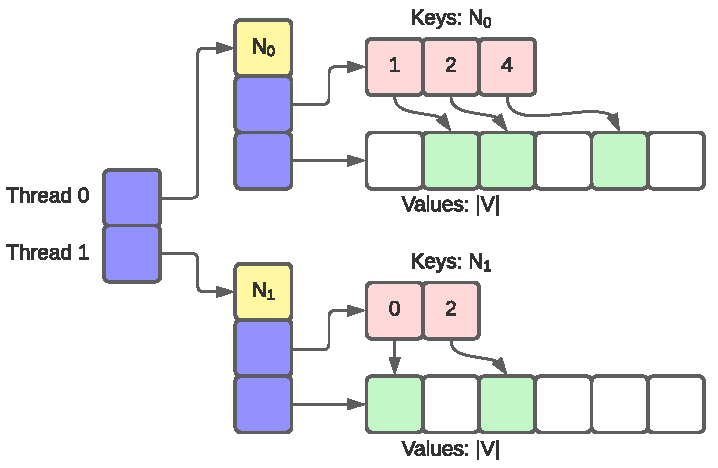
\includegraphics[width=0.88\linewidth]{out/louvainrak-hashtable.pdf}
  } \\[-2ex]
  \caption{TODO: Phase split of our \textit{Louvain} shown on the left, and pass split shown on the right.}
  \label{fig:louvainrak-hashtable}
\end{figure}

\begin{figure*}[hbtp]
  \centering
  \subfigure{
    \label{fig:louvain-pass--all}
    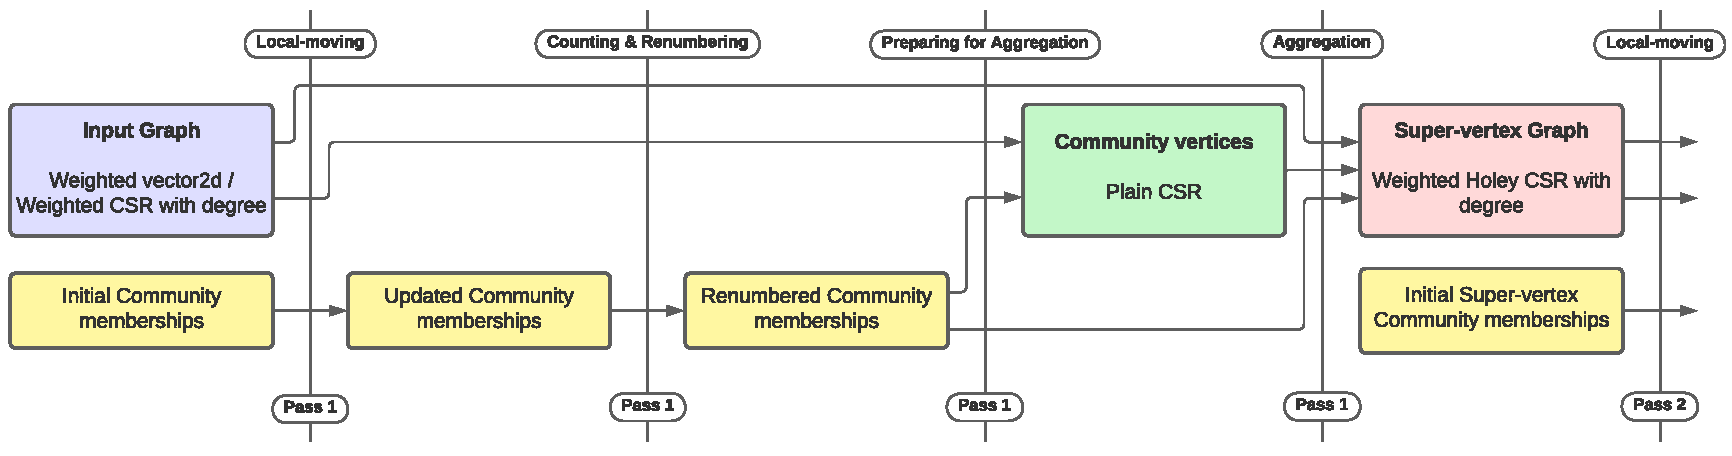
\includegraphics[width=0.98\linewidth]{out/louvain-pass.pdf}
  } \\[-2ex]
  \caption{A flow diagram illustrating the first pass of GVE-Louvain for a Weighted 2D-vector based or a Weighted CSR with degree based input graph. In the local-moving phase, vertex community memberships are updated until the total change in delta-modularity across all vertices reaches a specified threshold. Community memberships are then counted and renumbered. In the aggregation phase, community vertices in a CSR are first obtained. This is used to create the super-vertex graph stored in a Weighted Holey CSR with degree. In subsequent passes, the input is a Weighted Holey CSR with degree and initial community membership for super-vertices from the previous pass.}
  \label{fig:louvain-pass}
\end{figure*}
% A flow diagram showing the high level steps followed in the first pass of our Louvain implementation. The input graph is a weighted 2D vector based graph or weighted CSR with degree graph. In the local-moving phase, the community membership of each vertex is updated until the net change in delta-modularity across all vertices in an iteration reaches a threshold/tolerance. The community memberships are then counted and renumbered. In the aggregation phase of the algorithm, we obtain the vertices belonging to each community as a CSR, and later use this to generate the super-vertex graph. The super-vertex graph is stored in a weighted holey CSR with degree, i.e., the CSR is over-allocated with gaps between edges (ids and weights), and a degree vector is instead used to keep track of the degree of each super-vertex. In the remaining passes, the input graph is a weighted holey CSR with degree (from the previous pass) and an initial community membership vector for each super-vertex.
\begin{algorithm}[hbtp]
\caption{GVE-Louvain: Our parallel Louvain algorithm.}
\label{alg:louvain}
\begin{algorithmic}[1]
\Require{$G$: Input graph}
\Require{$C$: Community membership of each vertex}
\Require{$G'$: Input/super-vertex graph}
\Require{$C'$: Community membership of each vertex in $G'$}
\Require{$K'$: Total edge weight of each vertex}
\Require{$\Sigma'$: Total edge weight of each community}
\Ensure{$G'_{C'}$: Community vertices (CSR)}
\Ensure{$H_t$: Collision-free per-thread hashtable}
\Ensure{$l_i$: Number of iterations performed (per pass)}
\Ensure{$l_p$: Number of passes performed}
\Ensure{$\tau$: Per iteration tolerance}
\Ensure{$\tau_{agg}$: Aggregation tolerance}

\Statex

\Function{louvain}{$G$} \label{alg:louvain--begin}
  \State Vertex membership: $C \gets [0 .. |V|)$ \textbf{;} $G' \gets G$ \label{alg:louvain--initialization}
  \ForAll{$l_p \in [0 .. \text{\small{MAX\_PASSES}})$} \label{alg:louvain--passes-begin}
    \State $\Sigma' \gets K' \gets vertexWeights(G')$ \textbf{;} $C' \gets [0 .. |V'|)$ \label{alg:louvain--reset-weights}
    \State Mark all vertices in $G'$ as unprocessed \label{alg:louvain--reset-affected}
    \State $l_i \gets louvainMove(G', C', K', \Sigma')$ \Comment{Alg. \ref{alg:louvainlm}} \label{alg:louvain--local-move}
    \If{$l_i \le 1$} \textbf{break} \Comment{Globally converged?} \label{alg:louvain--globally-converged}
    \EndIf
    \State $|\Gamma|, |\Gamma_{old}| \gets$ Number of communities in $C$, $C'$
    \If{$|\Gamma|/|\Gamma_{old}| > \tau_{agg}$} \textbf{break} \Comment{Low shrink?} \label{alg:louvain--aggregation-tolerance}
    \EndIf
    \State $C' \gets$ Renumber communities in $C'$ \label{alg:louvain--renumber}
    \State $C \gets$ Lookup dendrogram using $C$ to $C'$ \label{alg:louvain--lookup}
    \State $G' \gets louvainAggregate(G', C')$ \Comment{Alg. \ref{alg:louvainag}} \label{alg:louvain--aggregate}
    \State $\tau \gets \tau / \text{\small{TOLERANCE\_DROP}}$ \Comment{Threshold scaling} \label{alg:louvain--threshold-scaling}
  \EndFor \label{alg:louvain--passes-end}
  \State $C \gets$ Lookup dendrogram using $C$ to $C'$ \label{alg:louvain--lookup-last}
  \Return{$C$} \label{alg:louvain--return}
\EndFunction \label{alg:louvain--end}
\end{algorithmic}
\end{algorithm}

\begin{algorithm}[hbtp]
\caption{Our parallel Label Propagation Algorithm (LPA).}
\label{alg:rak}
\begin{algorithmic}[1]
\Function{lpa}{$G$} \label{alg:rak--main-begin}
  \State Vertex membership: $C' \gets [0 .. |V|)$ \textbf{;} $G' \gets G$ \label{alg:rak--initialization}
  \State Mark all vertices in $G'$ as unprocessed
  \ForAll{$l_i \in [0 .. \text{\small{MAX\_ITERATIONS}})$} \label{alg:rak--iterations-begin}
    \State $\Delta N \gets lpaMove(G', C')$ \label{alg:rak--propagate}
    \If{$\Delta N/N \le \tau$} \textbf{break} \Comment{Converged?} \label{alg:rak--converged}
    \EndIf
  \EndFor \label{alg:rak--iterations-end}
  \Return{$C'$}
\EndFunction \label{alg:rak--main-end}

\Statex

\Function{lpaMove}{$G', C'$} \label{alg:rak--move-begin}
  \State Changed vertices: $\Delta N \gets 0$
  \ForAll{unprocessed $i \in V'$ \textbf{in parallel}}
    \State Mark $i$ as processed (prune) \label{alg:rak--prune}
    \State $c^* \gets$ Most weighted label to $i$ in $G'$ \label{alg:rak--best-community}
    \If{$c^* = C'[i]$} \textbf{continue} \label{alg:rak--best-community-same}
    \EndIf
    \State $C'[i] \gets c^*$ \textbf{;} $\Delta N \gets \Delta N + 1$ \label{alg:rak--perform-move}
    \State Mark neighbors of $i$ as unprocessed \label{alg:rak--remark}
  \EndFor
\Return{$\Delta N$}
\EndFunction \label{alg:rak--move-end}
\end{algorithmic}
\end{algorithm}




%% Parameter setting
% TOLERANCE = 0.05
% MAX\_ITERATIONS = 20
% MAX\_THREADS = 12

\begin{figure*}[hbtp]
  \centering
  \subfigure{
    \label{fig:louvain-opt--all}
    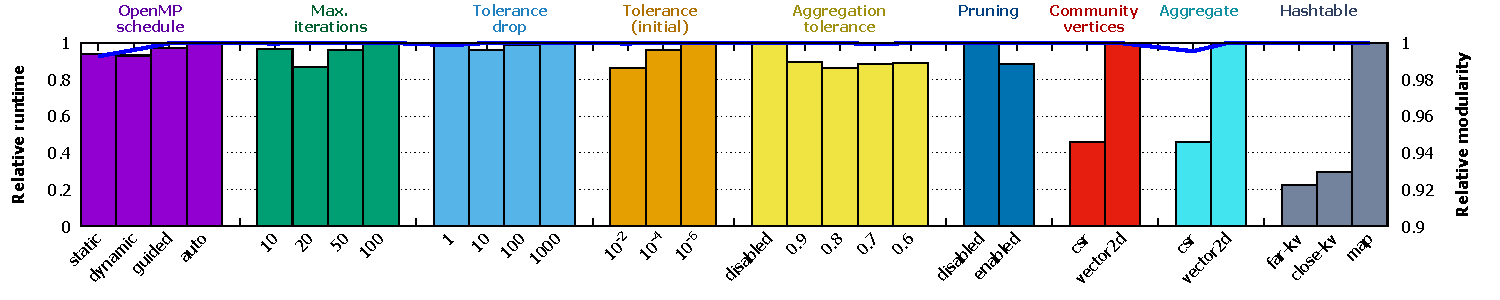
\includegraphics[width=0.98\linewidth]{out/louvain-opt.pdf}
  } \\[-2ex]
  \caption{Impact of various parameter controls and optimizations on the runtime and result quality (modularity) of the \Lou{} algorithm. We show the impact of each optimization upon the relative runtime on the left Y-axis, and upon the relative modularity on the right Y-axis.}
  \label{fig:louvain-opt}
\end{figure*}

\begin{figure*}[hbtp]
  \centering
  \subfigure{
    \label{fig:rak-opt--all}
    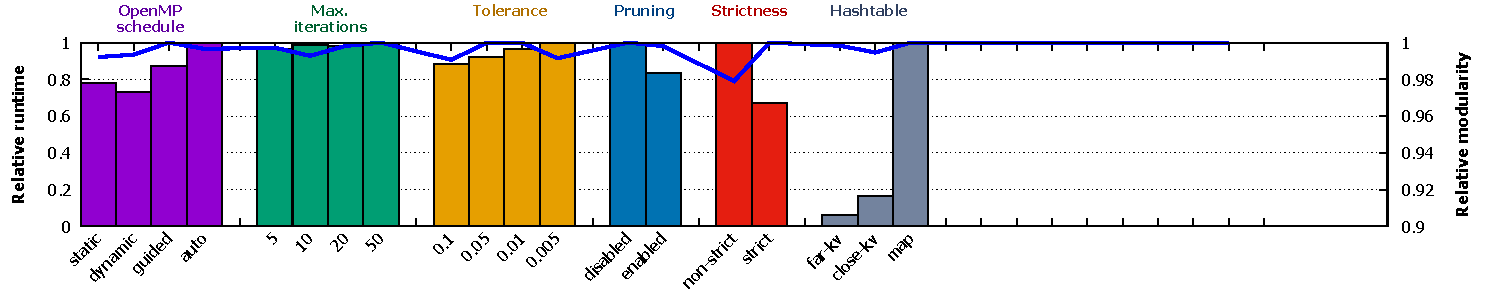
\includegraphics[width=0.98\linewidth]{out/rak-opt.pdf}
  } \\[-2ex]
  \caption{Impact of various parameter controls and optimizations on the runtime and result quality (modularity) of the \LPA{}. Again, we show the impact of each optimization upon the relative runtime on the left Y-axis, and upon the relative modularity on the right Y-axis.}
  \label{fig:rak-opt}
\end{figure*}


We use a parallel implementation of the Louvain method to determine suitable parameter settings and optimize the original algorithm through experimentation with a variety of techniques. We use \textit{asynchronous} version of Louvain, where threads work independently on different parts of the graph. This allows for faster convergence but can also lead to more variability in the final result \cite{com-blondel08, com-halappanavar17}. Further, we allocate a separate hashtable per thread to keep track of the delta-modularity of moving to each community linked to a vertex in the local-moving phase of the algorithm, and to keep track of the total edge weight from one super-vertex to the other super-vertices in the aggregation phase of the algorithm.

Our optimizations include using OpenMP's \verb|dynamic| loop schedule, limiting the number of iterations per pass to $20$, using a tolerance drop rate of $10$, setting an initial tolerance of $0.01$, using an aggregation tolerance of $0.8$, employing vertex pruning, making use of parallel prefix sum and preallocated Compressed Sparse Row (CSR) data structures for finding community vertices and for storing the super-vertex graph during the aggregation phase, and using fast collision-free per-thread hashtables which are well separated in their memory addresses (\textit{Far-KV}) for the local-moving and aggregation phases of the algorithm. Details on each of the optimizations is given below.

For each optimization, we test a number of relevant alternatives, and show the relative time and the relative modularity of communities obtained by each alternative in Figure \ref{fig:louvain-opt}. This result is obtained the running the tests on each graph in the dataset (see Table \ref{tab:dataset}), $5$ times on each graph to reduce the impact of noise, taking their geometric mean and arithmetic mean for the runtime and modularity respectively, and representing them as a ratio within each optimization category.

\begin{figure*}[hbtp]
  \centering
  \subfigure{
    \label{fig:louvainrak-sta--all}
    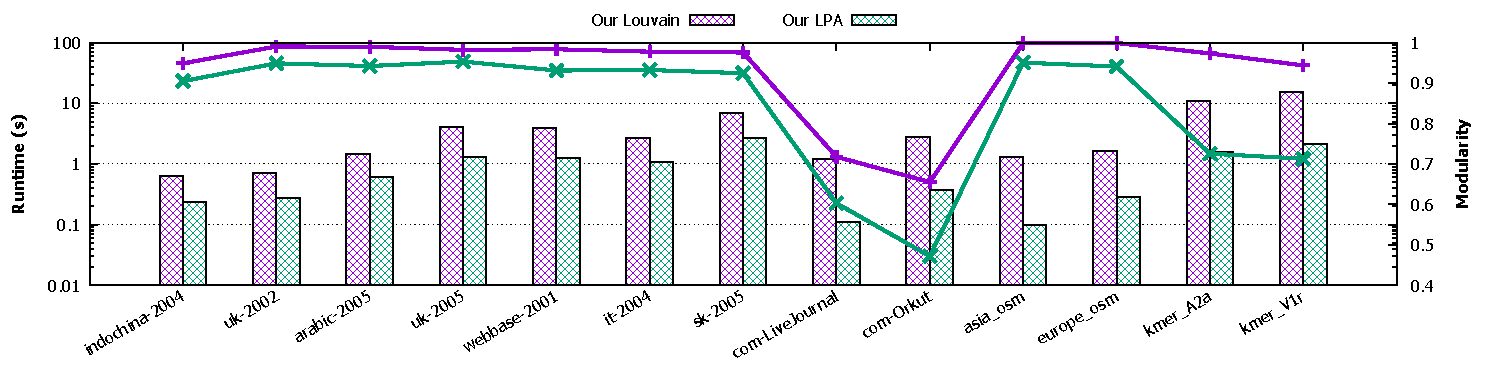
\includegraphics[width=0.98\linewidth]{out/louvainrak-sta.pdf}
  } \\[-2ex]
  \caption{Time taken (boxes), and modularity of communities obtained (lines) with our \textit{Louvain} and \textit{LPA} for each graph in the dataset. Runtime is shown with logarithmic scale on the left Y-axis (in seconds), and modularity is shown with linear scale on the right Y-axis.}
  \label{fig:louvainrak-sta}
\end{figure*}

\begin{figure*}[hbtp]
  \centering
  \subfigure{
    \label{fig:louvainrak-stas--all}
    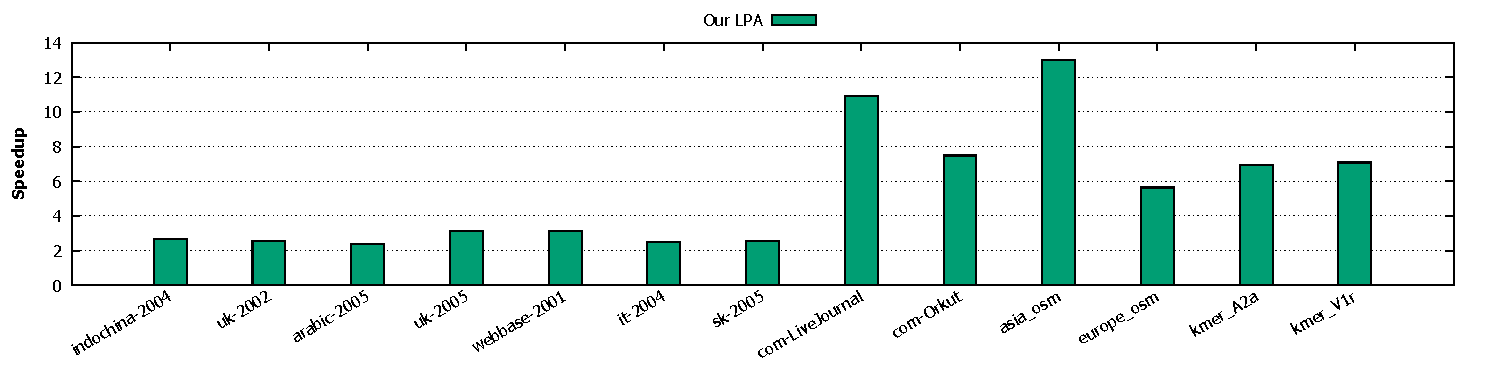
\includegraphics[width=0.98\linewidth]{out/louvainrak-stas.pdf}
  } \\[-2ex]
  \caption{Speedup of our \textit{LPA} with respect to our \textit{Louvain} for each graph in the dataset.}
  \label{fig:louvainrak-stas}
\end{figure*}

\begin{figure*}[hbtp]
  \centering
  \subfigure[Our Louvain]{
    \label{fig:louvainrak-hardness--louvain}
    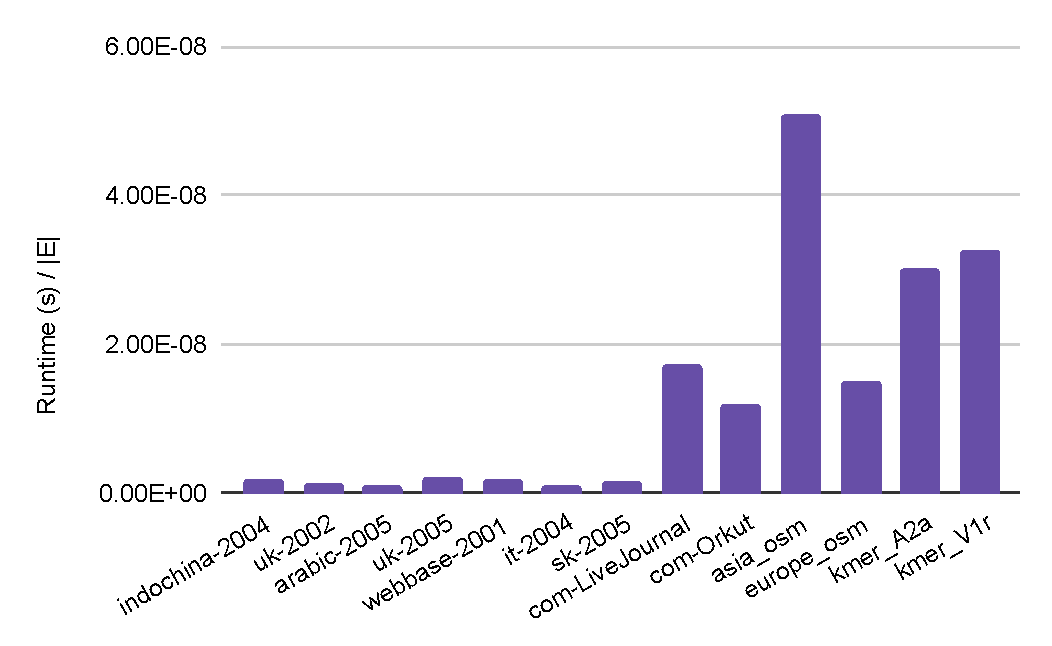
\includegraphics[width=0.48\linewidth]{out/louvain-hardness.pdf}
  }
  \subfigure[Our LPA]{
    \label{fig:louvainrak-hardness--rak}
    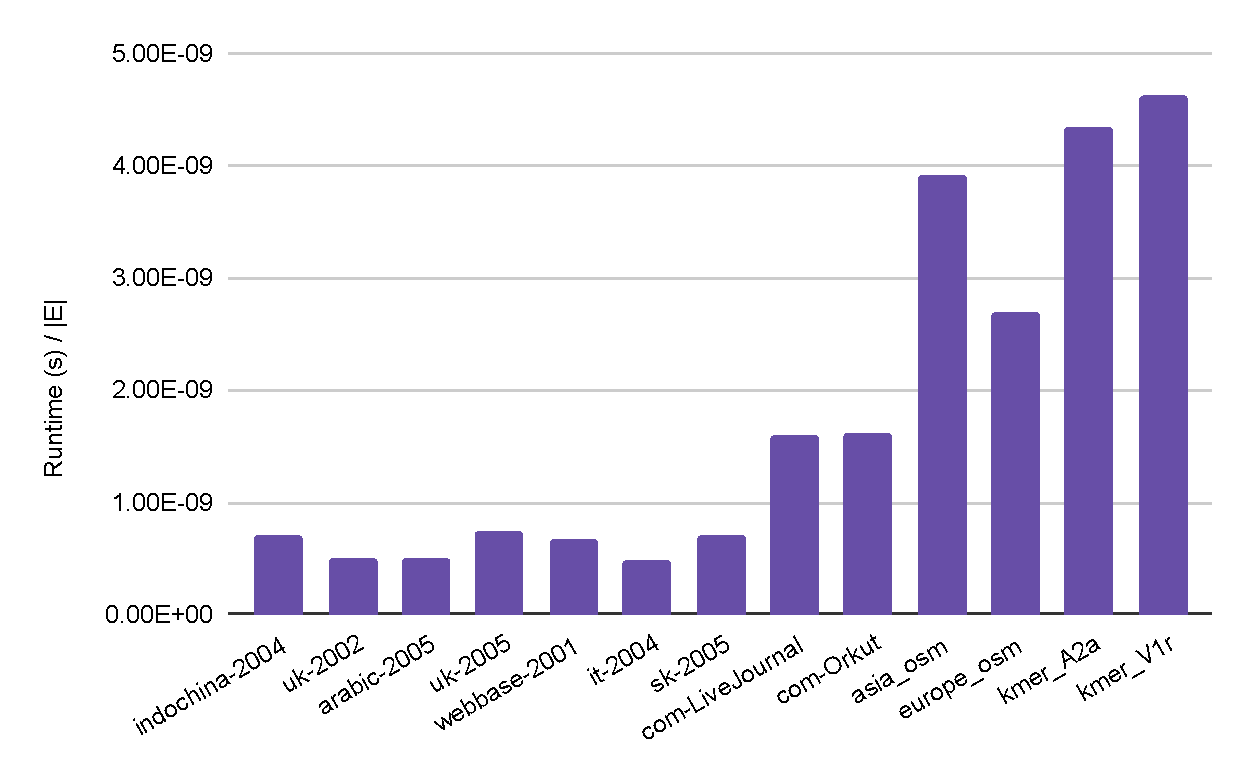
\includegraphics[width=0.48\linewidth]{out/rak-hardness.pdf}
  } \\[-2ex]
  \caption{Runtime $/ |E|$ with our \textit{Louvain} shown on the left, and runtime $/ |E|$ with our \textit{LPA} shown on the right.}
  \label{fig:louvainrak-hardness}
\end{figure*}



\subsubsection{Adjusting OpenMP loop schedule}

We attempt \textit{static}, \textit{dynamic}, \textit{guided}, and \textit{auto} loop scheduling approaches of OpenMP (each with a chunk size of $2048$) to parallelize the local-moving and aggregation phases of the Louvain algorithm. Results indicate that the scheduling behavior can have small impact on the quality of obtained communities. We consider OpenMP's \verb|dynamic| loop schedule to be the best choice, as it helps achieve better load balancing when the degree distribution of vertices is non-uniform, and offers a $7\%$ reduction in runtime with respect to OpenMP's \textit{auto} loop schedule, with only a $0.4\%$ reduction in the modularity of communities obtained (which is likely to be just noise).

\subsubsection{Limiting the number of iterations per pass}

Restricting the number of iterations of the local-moving phase ensures its termination within a reasonable number of iterations, which helps minimize runtime. This can be important since the local-moving phase performed in the first pass is the most expensive step of the algorithm. However, choosing too small a limit may worsen convergence rate. Our results indicate that limiting the maximum number of iterations to $20$ allows for $13\%$ faster convergence, when compared to a maximum iterations of $100$.


\subsubsection{Adjusting tolerance drop rate (threshold scaling)}

Tolerance is used to detect convergence in the local-moving phase of the Louvain algorithm, i.e., when the total delta-modularity in a given iteration is below or equal to the specified tolerance, the local-moving phase is considered to have converged. Instead of using a fixed tolerance across all passes of the Louvain algorithm, we can start with an initial high tolerance and then gradually reduce it. This is known as threshold scaling \cite{com-lu15, com-naim17, com-halappanavar17}, and it helps minimize runtime as the first pass of the algorithm (which is usually the most expensive). Based on our findings, a tolerance drop rate of $10$ yields $4\%$ faster convergence, with respect to a tolerance drop rate of $1$ (threshold scaling disabled), with no reduction in quality of communities obtained.


\subsubsection{Adjusting initial tolerance}

Starting with a smaller initial tolerance allows the algorithm to explore broader possibilities for community assignments in the early stage, but comes at the cost of increased runtime. We find an initial tolerance of $0.01$ provides a $14\%$ reduction in runtime of the algorithm with no reduction in the quality of identified communities, when compared to an initial tolerance of $10^{-6}$.


\subsubsection{Adjusting aggregation tolerance}

The aggregation tolerance determines the point at which communities are considered to have converged based on the number of community merges. In other words, if too few communities merged this pass we should stop here, i.e., if $|V_{aggregated}|/|V| \geq$ aggregation tolerance, we consider the algorithm to have converged. Adjusting aggregation tolerance allows the algorithm to stop earlier when further merges have minimal impact on the final result. According to our observations, an aggregation tolerance of $0.8$ appears to be the best choice, as it presents a $14\%$ reduction in runtime, when compared to the aggregation tolerance being disabled ($1$), while identifying final communities of equivalent quality.


\subsubsection{Vertex pruning}

Vertex pruning is a technique that is used to minimize unnecessary computation. Here, when a vertex changes its community, its marks its neighbors to be processed. Once a vertex has been processed, it is marked as not to be processed. However, it comes with an added overhead of marking an unmarking of vertices. Based on our results, vertex pruning justifies this overhead, and should be enabled for $11\%$ improvement in performance.

\begin{figure*}[hbtp]
  \centering
  \subfigure[Phase split]{
    \label{fig:louvain-splits--phase}
    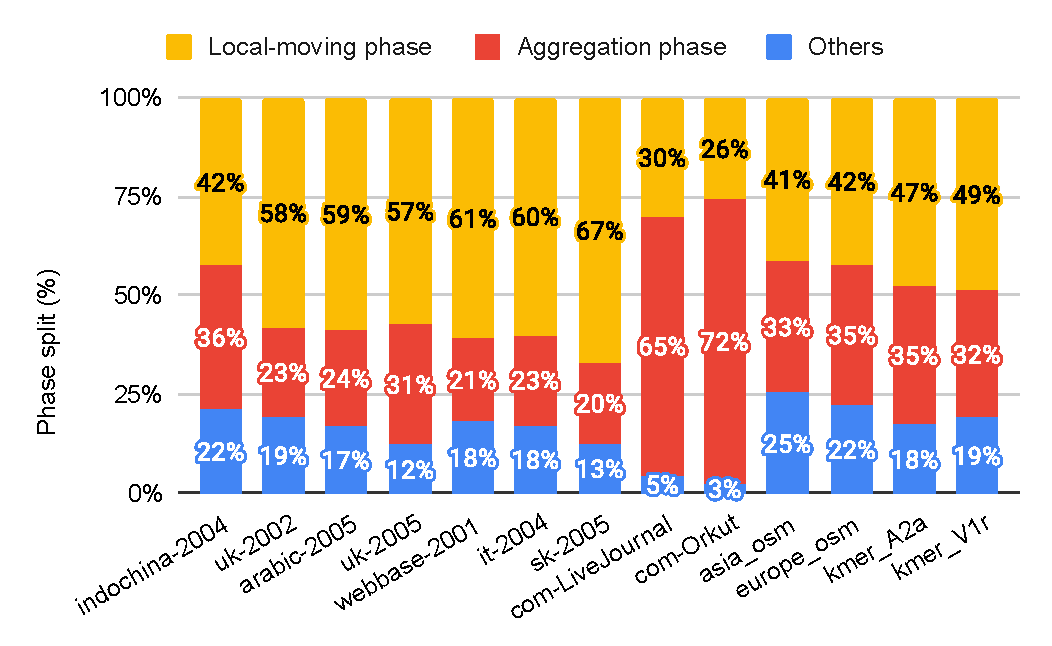
\includegraphics[width=0.48\linewidth]{out/louvain-phases.pdf}
  }
  \subfigure[Pass split]{
    \label{fig:louvain-splits--pass}
    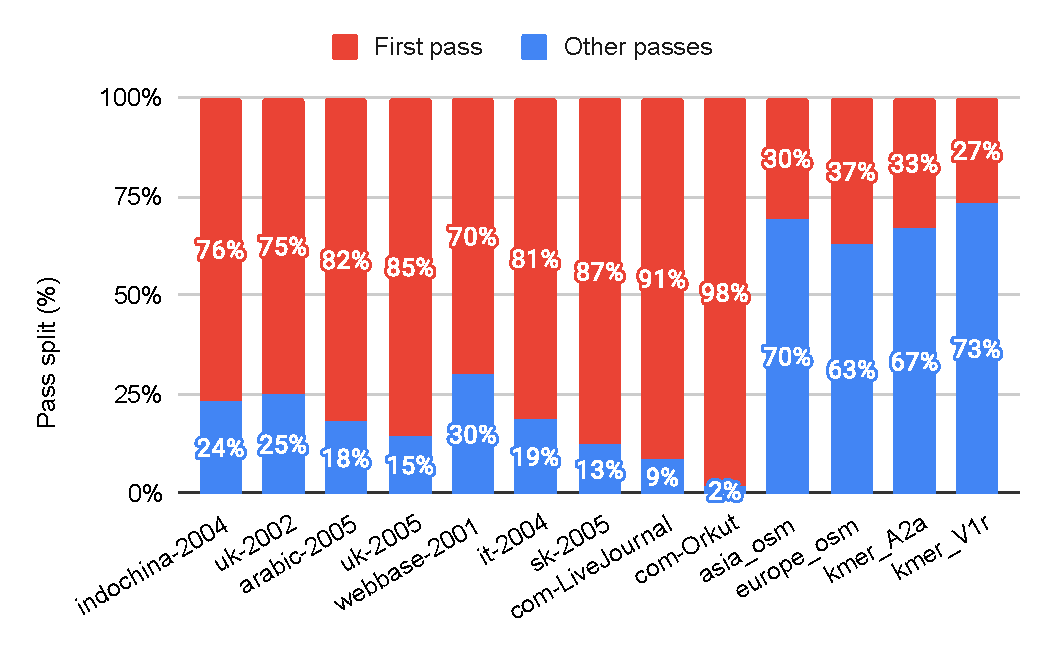
\includegraphics[width=0.48\linewidth]{out/louvain-passes.pdf}
  } \\[-2ex]
  \caption{Phase split of \textit{GVE-Louvain} shown on the left, and pass split shown on the right for each graph in the dataset.}
  \label{fig:louvain-splits}
\end{figure*}



\subsubsection{Finding community vertices for aggregation phase}

In the aggregation phase of the Louvain algorithm, the communities obtained in the previous local-moving phase of the algorithm are combined into super-vertices in the aggregated graph, with the edges between two super-vertices being equal to the total weight of edges between the respective communities. This requires one to obtain the list of vertices belonging to each community, instead of the mapping of community membership of each vertex that we have after the local-moving phase ends. A straight-forward implementation of this would make use of two-dimensional arrays for storing vertices belonging to each community, with the index in the first dimension representing the community id $c$, and the index in the second dimension pointing to the $n^{th}$ vertex in the given community $c$. However, this requires memory allocation during the algorithm, which is expensive. Employing a parallel prefix sum technique along with a preallocated Compressed Sparse Row (CSR) data structure eliminates repeated memory allocation and deallocation, enhancing performance. Indeed, out findings indicate that using parallel prefix sum along with a preallocated CSR is $2.2\times$ faster than using 2D arrays for aggregating vertices.


\subsubsection{Storing aggregated communities (super-vertex graph)}

After the list of vertices belonging to each community have been obtained, the communities need to be aggregated (or compressed) into super-vertices, such that edges between two super-vertices being equal to the total weight of edges between the respective communities. This is generally called the super-vertex graph, or the compressed graph. It is then used as an input to the local-moving phase of the next pass of the Louvain algorithm. A simple data structure to store the super-vertex graph in the adjacency list format would be a two-dimensional array. Again, this requires memory allocation during the algorithm, which is bad for performance. Utilizing two preallocated CSRs, one for the source graph and the other for the target graph (except the first pass, where the dynamic graph may be stored in any desired format suitable for dynamic batch updates), along with parallel prefix sum can help here. We observe that using parallel prefix sum along with preallocated CSRs for maintaining the super-vertex graph is again $2.2\times$ faster than using 2D arrays.


\subsubsection{Hashtable design for local-moving/aggregation phases}

One can use C++'s inbuilt maps as per-thread (independent) hashtables for the Louvain algorithm. But this has poor performance. So we use a key-list and a full-size values array (collision-free) to dramatically improve performance. However, if the memory addresses of the hashtables are nearby (\textit{Close-KV}), even if each thread uses its own hashtable exclusively, performance is not as high. This is possibly due to false cache-sharing. Alternatively, if we ensure that the memory address of each hashtable are farther away (\textit{Far-KV}), the performance improves. Our results indicate that \textit{Far-KV} has the best performance and is $4.4\times$ faster than \textit{Map}, and $1.3\times$ faster than \textit{Close-KV} hashtable implementations.


\subsubsection{Results with optimized implementation}

The combined optimizations yield impressive performance improvements in the OpenMP-based \StaLou{}, with a completion time of $6.8$ seconds on the \textit{sk-2005} graph containing $3.8 B$ edges (refer to Figure \ref{fig:louvainrak-sta}). We observe that graphs with lower average degree (\textit{road networks} and \textit{protein k-mer graphs}) and graphs with poor community structure (such as \verb|com-LiveJournal| and \verb|com-Orkut|) have a larger $\text{runtime}/|E|$ factor, as shown in Figure \ref{fig:louvainrak-hardness--louvain}.

The phase-wise and pass-wise split of the optimized \StaLou{} is shown in Figure \ref{fig:louvain-splits}. Note how $48\%$ (most) of the runtime of the algorithm is spent in the local-moving phase, while only $29\%$ of the runtime is spent in the aggregation phase of the algorithm. Further, $68\%$ (most) of the runtime is spent in the first pass of the algorithm, which is the most expensive pass due to the size of the original graph (later passes work on super-vertex graphs) \cite{com-wickramaarachchi14}.




\subsection{Our Parallel LPA implementation}
\label{sec:rak}

Like Louvain, we use a parallel implementation of LPA and experiment with different optimizations and parameter settings. Again, as with Louvain, we use the \textit{asynchronous} version of LPA. We observe that parallel LPA obtains communities of higher quality than its sequential implementation, possibly due to randomization. Further, we allocate a separate hash table per thread, as with the Louvain algorithm. In LPA, the hashtable is used to keep track of the total weight of each unique label linked to a vertex.

For LPA, our optimizations include using OpenMP's \verb|dynamic| loop schedule, setting an initial tolerance of $0.05$, enabling vertex pruning, employing the strict version of LPA, and using fast collision-free per-thread hashtables which are well separated in their memory addresses (\textit{Far-KV}). See below for the details on each optimization. We evaluate multiple alternatives for each optimization, and show the relative time and the relative modularity of communities obtained by each alternative in Figure \ref{fig:rak-opt}. Similar to Louvain, we perform these tests on every graph in the dataset (refer to Table \ref{tab:dataset}), conducting them five times on each graph to minimize the influence of noise. We then calculate the geometric mean for the runtime and arithmetic mean for the modularity, and represent them as ratios within each optimization category.


\subsubsection{Adjusting OpenMP loop schedule}

We attempt \textit{static}, \textit{dynamic}, \textit{guided}, and \textit{auto} loop scheduling approaches of OpenMP (each with a chunk size of $2048$) to parallelize LPA. Similar to the Louvain method, we consider OpenMP's \verb|dynamic| loop schedule to be the best choice, due to its ability of work balancing among threads, and because it yields a runtime reduction of $27\%$ when compared to OpenMP's \textit{auto} loop schedule, while incurring only a $0.7\%$ reduction in the modularity of obtained communities (which again is likely to be just noise).


\subsubsection{Limiting the number of iterations}

Restricting the number of iterations of LPA can ensure its termination within a reasonable number of iterations, but choosing a small limit may worsen the quality of communities obtained. Our results suggest that limiting the maximum number of iterations to $20$ strikes a good balance between runtime and modularity.


\subsubsection{Adjusting tolerance}

Using a small tolerance allows the algorithm to explore broader possibilities for community assignments, but comes at the cost of increased runtime. We find an initial tolerance of $0.05$ to be suitable. A tolerance of $0.1$ may also be acceptable, but provides a very small gain in performance when compared to a tolerance of $0.05$.


\subsubsection{Vertex pruning}

Vertex pruning is a method utilized to minimize unnecessary computation. In this approach, when a vertex alters its community, it assigns its neighbors for processing. Once a vertex has been processed, it is labeled as ineligible for further processing. However, this procedure incurs an additional overhead due to the marking and unmarking of vertices. Based on our findings, the employment of vertex pruning justifies this overhead and results in a performance enhancement of $17\%$.


\subsubsection{Picking the best label}

When there exist multiple labels connected to a vertex with maximum weight, we may randomly pick one of them (non-strict LPA), or pick only the first of them (strict LPA). We implement non-strict LPA using a simple modulo operator on the label id, as we observe that using \textit{xorshift} based random number generator does not provide any advantage. Results indicate that the strict version of LPA is $1.5\times$ faster than the non-strict approach, while also offering a gain in modularity of $2.1\%$.


\subsubsection{Hashtable design}

One can utilize C++'s inbuilt map as per-thread (independent) hashtables for the LPA algorithm. However, as mentioned before, this exhibits poor performance. Therefore, we employ a key-list and a collision-free full-size values array to dramatically improve performance. However, if the memory addresses of the hashtables are nearby (\textit{Close-KV}), even if each thread uses its own hashtable exclusively, the performance is not as high. This is possibly due to false cache-sharing. Alternatively, if we ensure that the memory address of each hashtable is farther away (\textit{Far-KV}), the performance improves. Our results indicate that \textit{Far-KV} has the best performance and is $15.8\times$ times faster than \textit{Map}, and $2.6\times$ times faster than \textit{Close-KV} with LPA.


\subsubsection{Results with optimized implementation}

The combined optimizations result in high performance of the OpenMP-based \StaLPA{} (see Figure \ref{fig:louvainrak-sta}). It has a runtime of $2.7$ seconds on the \textit{sk-2005} graph containing $3.8 B$ edges. We observe, as shown in Figure \ref{fig:louvainrak-hardness--rak}, that graphs with lower average degree (\textit{road networks} and \textit{protein k-mer graphs}) have a larger $\text{runtime}/|E|$ factor.
